\documentclass{beamer}

\usepackage[english]{babel}
\usepackage[utf8]{inputenc}
%\usepackage[plainpages=false,pdfpagelabels,unicode]{hyperref}
\usepackage{graphicx}
\usepackage{pdfpages}

\usetheme{Warsaw}

\begin{document}

\title[Ti$_x$Si$_{1-x}$O$_2$ work, short summary] % (optional, only for long titles)
{TiSiO$_2$ work, short summary}
\subtitle{Short summary}
\author{Pavel Ondračka}
%\institute
%{
%	 Faculty of Science, Masaryk University\\
%	Brno, Czech Republic
%  \and
%	CEITEC - Central European Institute of Technology\\
%	Brno, Czech Republic
%}
\date{25.08.2015}

\maketitle

%\begin{frame}
%	\frametitle{Outline}
%  \tableofcontents
%\end{frame}


\begin{frame}
\frametitle{Available samples}

\begin{table}
	\begin{centering}
	\begin{tabular}{lccc}
		\hline
		& N27BS & N25BS & N23BS\\
		\hline \hline
		\% O & 57.2 & 63.4 & 64.4\\
		\% Ti & 25.1 & 18.0 & 13.7\\
		\% Si & 0.0 & 11.4 & 16.5\\
		\% C & 6.3 & 0.5 & 0.5 \\
		\% H & 11.4 & 6.8 & 4.9\\
		$x$ ([Si]/[Si]+[Ti]) & 0 & 0.39 & 0.55\\
 		\hline
	\end{tabular}
	\caption{Film composition (atomic \%) measured by RBS/ERDA}
	\label{RBS}
	\end{centering}
\end{table}


\end{frame}

\begin{frame}
\frametitle{Structural properties - experiment}
\begin{center}
	\includegraphics[width=0.8\linewidth]{figures/all.pdf}
\end{center}
\begin{center}
	\includegraphics[width=0.8\linewidth]{figures/anatase-XRD.pdf}
\end{center}
\end{frame}

\begin{frame}
\frametitle{Structural properties - calculations}
	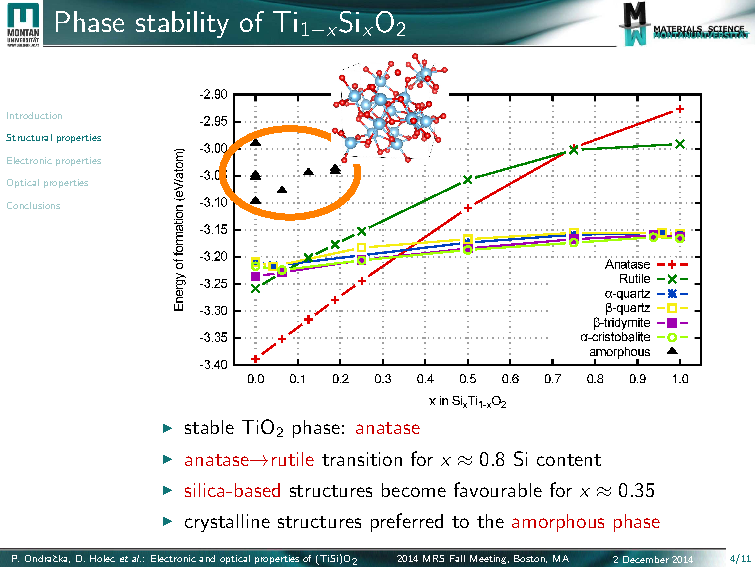
\includegraphics[width=\linewidth]{figures/stability.pdf}
\end{frame}

\begin{frame}
\frametitle{Calculated optical constants}
	\includegraphics[width=\linewidth]{figures/SiTiO2-eps.pdf}
\end{frame}

\begin{frame}
\frametitle{Optical constants - comparison}
	\includegraphics[width=\linewidth]{figures/compare.pdf}
\end{frame}

\begin{frame}
\frametitle{Band gap}
	\includegraphics[width=\linewidth]{figures/gap.pdf}
\end{frame}

\begin{frame}
\frametitle{Current work}
\begin{itemize}
   \item Better amourphous models (96 vs 48 atoms) + different simulated annealing recipes.
   \item how to obtain ,,band gap'' comparable with experiment from amorphous cells
   \item Si and Ti mixing, FTIR unconclusive, awaiting results from HRTEM
\end{itemize}
\end{frame}

\end{document}
